\begin{figure}[htb]
    \vspace{-0.1cm}
    \begin{center}
    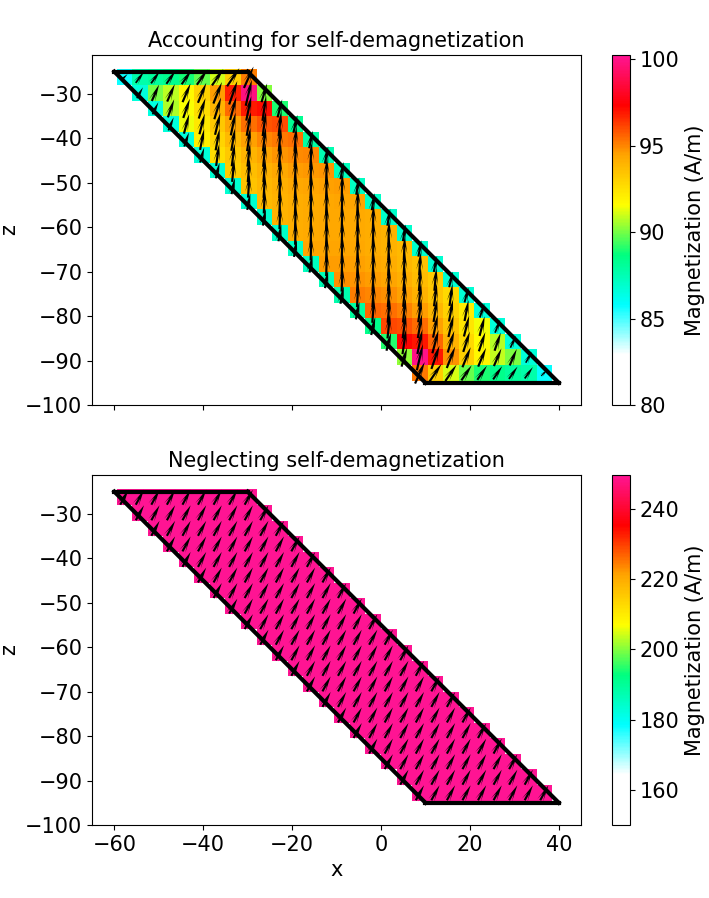
\includegraphics[width=\columnwidth]{figures/Magnetization.png}
    \end{center}
    \vspace{-0.5cm}
\caption{
    Computed magnetizations of a plate when accounting for self-demagnetization using the non-linear code (top panel) and when neglecting self demagnetization using the standard linear susceptibility code (bottom panel).
}
\label{fig:magnetization}
\vspace{-0.1cm}
\end{figure}

